\chapter{Ensembles de nombres et intervalles}

\section{Ensembles de nombres}

\subsection{L'ensemble des entiers naturels $\N$}

\begin{df}
	\nline
	\begin{wrapstuff}[r,width=3cm]
		\begin{center}
			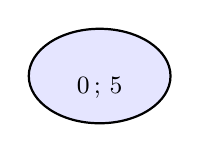
\begin{tikzpicture}[scale=0.75]
				\draw[thick, fill=blue!10] (0,0) ellipse (1.2cm and 0.8cm);
				\node at (0,0.3) {\textbf{$\N$}};
				\node[font=\small] at (0,-0.2) {$0 \,;\, 5$};
			\end{tikzpicture}
		\end{center}
	\end{wrapstuff}

	L'\textbf{ensemble des entiers naturels}, noté $\N$, est l'ensemble des entiers positifs ou nuls.
	\[
		\N = \{0\,;\, 1\,;\, 2\,;\, 3\,;\, 4\,;\, \dots\}
	\]
\end{df}

\begin{ex}
	$5 \in \N$ \quad et \quad $0 \in \N$.
\end{ex}

\subsection{L'ensemble des entiers relatifs $\Z$}

\begin{df}
	\nline
	\begin{wrapstuff}[r,width=4cm]
		\begin{center}
			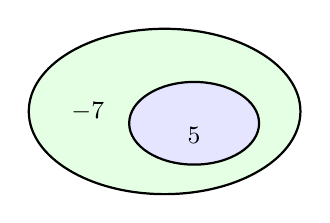
\begin{tikzpicture}[scale=0.75]
				\draw[thick, fill=green!10] (0,0) ellipse (2.3cm and 1.4cm);
				\node at (0,1) {\textbf{$\Z$}};
				\node[font=\small] at (-1.3,0) {$-7$};
				\draw[thick, fill=blue!10] (0.5,-0.2) ellipse (1.1cm and 0.7cm);
				\node at (0.5,0.05) {\textbf{$\N$}};
				\node[font=\small] at (0.5,-0.4) {$5$};
			\end{tikzpicture}
			\vspace*{-10mm}
		\end{center}
	\end{wrapstuff}
	L'\textbf{ensemble des entiers relatifs}, noté $\Z$, est l'ensemble des entiers positifs, négatifs ou nuls.
	\[
		\Z = \{\dots\,;\, - 3\,;\, - 2\,;\, - 1\,;\, 0\,;\, 1\,;\, 2\,;\, 3\,;\, \dots\}
	\]
\end{df}

\begin{ex}
	$-7 \in \Z$ \quad et \quad $5 \in \Z$ (tout entier naturel est aussi un entier relatif).
\end{ex}

\subsection{L'ensemble des nombres décimaux $\D$}

\begin{df}
	\nline
	\begin{wrapstuff}[r,width=5cm]
		\begin{center}
			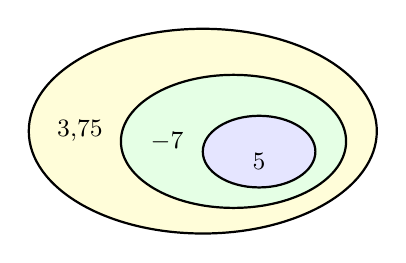
\begin{tikzpicture}[scale=0.65]
				\draw[thick, fill=yellow!15] (0,0) ellipse (3.4cm and 2cm);
				\node at (0,1.5) {\textbf{$\D$}};
				\node[font=\small] at (-2.4,0) {$3{,}75$};
				\draw[thick, fill=green!10] (0.6,-0.2) ellipse (2.2cm and 1.3cm);
				\node at (0.6,0.7) {\textbf{$\Z$}};
				\node[font=\small] at (-0.7,-0.2) {$-7$};
				\draw[thick, fill=blue!10] (1.1,-0.4) ellipse (1.1cm and 0.7cm);
				\node at (1.1,-0.15) {\textbf{$\N$}};
				\node[font=\small] at (1.1,-0.6) {$5$};
			\end{tikzpicture}
			\vspace*{-20mm}
		\end{center}
	\end{wrapstuff}

	L'\textbf{ensemble des nombres décimaux}, noté $\D$, est l'ensemble des nombres qui peuvent s'écrire sous la forme $\frac{a}{10^n}$, où $a \in \Z$ et $n \in \N$.

\end{df}

\begin{remarque}
	Un nombre décimal possède un \textbf{nombre fini de chiffres après la virgule}.
\end{remarque}

\begin{ex}
	$3{,}75 \in \D$ \quad car \quad $3{,}75 = \dfrac{375}{10^2}$
\end{ex}

\subsection{L'ensemble des nombres rationnels $\Q$}

\begin{df}
	\nline
	\begin{wrapstuff}[r,width=5.7cm]
		\begin{center}
			\begin{tikzpicture}[scale=0.55]
				\draw[thick, fill=orange!15] (0,0) ellipse (4.5cm and 2.6cm);
				\node at (0,2.1) {\textbf{$\Q$}};
				\node[font=\small] at (-3.2,0) {$\dfrac{1}{3}$};
				\draw[thick, fill=yellow!15] (0.7,-0.2) ellipse (3.3cm and 1.9cm);
				\node at (0.7,1.3) {\textbf{$\D$}};
				\node[font=\small] at (-1.7,-0.2) {$3{,}75$};
				\draw[thick, fill=green!10] (1.3,-0.4) ellipse (2.2cm and 1.2cm);
				\node at (1.3,0.4) {\textbf{$\Z$}};
				\node[font=\small] at (0,-0.4) {$-7$};
				\draw[thick, fill=blue!10] (1.8,-0.6) ellipse (1cm and 0.6cm);
				\node at (1.8,-0.35) {\textbf{$\N$}};
				\node[font=\small] at (1.8,-0.87) {$5$};
			\end{tikzpicture}
		\end{center}
		\vspace*{-10mm}
	\end{wrapstuff}

	L'\textbf{ensemble des nombres rationnels}, noté $\Q$, est l'ensemble des nombres qui peuvent s'écrire sous la forme d'une fraction $\frac{a}{b}$, avec $a \in \Z$ et $b \in \Z^*$ ($b \neq 0$).

	Son écriture décimale possède une \textbf{suite de chiffres qui se répète périodiquement} après la virgule.
\end{df}

\begin{ex}
	$\dfrac{1}{3} \in \Q$ \quad car \quad $\dfrac{1}{3} = 0{,}3333\dots$ (non décimal, mais rationnel ... voir démonstration ci-dessous).
\end{ex}

\begin{demo}[$\frac{1}{3}$ n'est pas un nombre décimal]
	On effectue un raisonnement par l'absurde.

	Supposons que $\tfrac{1}{3}$ soit un nombre décimal.

	Alors, par définition, il pourrait s'écrire sous la forme :

	\[
		\frac{1}{3} = \frac{a}{10^n} \quad \text{avec } a \in \Z \text{ et } n \in \N
	\]

	En effectuant le produit en croix, on obtient :

	\[
		3 \times a = 10^n \times 1 \implies 3a = 10^n
	\]

	Cela signifie que $10^n$ doit être un multiple de $3$.

	Or, un nombre est divisible par $3$ si la somme de ses chiffres est un multiple de $3$.

	La somme des chiffres de $10^n$ (qui s'écrit $1$ suivi de $n$ zéro(s)) est égale à $1 + 0 + \dots + 0 = 1$.

	Puisque $1$ n'est pas divisible par $3$, $10^n$ n'est jamais un multiple de $3$.

	Nous obtenons une \textbf{contradiction}.

	L'hypothèse de départ est donc fausse : $\frac{1}{3}$ n'est pas un nombre décimal $\pa{\frac{1}{3} \notin \D}$.
\end{demo}

\subsection{L'ensemble des nombres réels $\R$}

\begin{df}
	L'\textbf{ensemble des nombres réels}, noté $\R$, est l'ensemble de tous les nombres connus en Seconde (représentés par tous les points de la droite graduée).

	Il contient les nombres rationnels ainsi que les \textbf{nombres irrationnels}, qui ne peuvent pas s'écrire sous forme de fraction.
\end{df}

\begin{ex}
	$\sqrt{2} \in \R$ \quad et \quad $\pi \in \R$ \quad (ce sont des nombres irrationnels).
\end{ex}

\begin{demo}[$\sqrt{2}$ n'est pas un nombre rationnel]

	On effectue à nouveau un raisonnement par l'absurde.

	Supposons que $\sqrt{2}$ soit un nombre rationnel.

	Alors $\sqrt{2}$ s'écrit sous la forme d'une fraction irréductible :

	\[
		\sqrt{2} = \frac{a}{b} \quad \text{avec } a \in \N^*, b \in \N^*
	\]

	En élevant au carré des deux côtés :

	\[
		2 = \frac{a^2}{b^2} \implies a^2 = 2b^2
	\]

	Comme $a^2$ s'écrit sous la forme $2k$ (avec $k = b^2$), $a^2$ est un nombre \textbf{pair}.

	Or, le carré d'un nombre impair est impair. Ainsi, comme $a^2$ est pair, \textbf{$a$ est nécessairement pair}.

	Puisque $a$ est pair, il existe un entier $k \in \N^*$ tel que $a = 2k$.

	En remplaçant dans l'égalité $a^2 = 2b^2$ :

	\[
		(2k)^2 = 2b^2 \implies 4k^2 = 2b^2 \implies b^2 = 2k^2
	\]

	De même, $b^2$ s'écrit $2k^2$, donc $b^2$ est pair, ce qui implique que \textbf{$b$ est aussi pair}.

	Si $a$ et $b$ sont tous les deux pairs, ils sont tous les deux divisibles par $2$.

	Cela contredit le fait que $\dfrac{a}{b}$ est irréductible.

	Nous obtenons une \textbf{contradiction}.

	L'hypothèse de départ est donc fausse : $\sqrt{2}$ n'est pas un nombre rationnel ($\sqrt{2} \notin \Q$).
\end{demo}

\begin{prop}[Inclusion globale des ensembles de nombres]

	\[
		\N \subset \Z \subset \D \subset \Q \subset \R
	\]

\end{prop}

\begin{center}
	\begin{tikzpicture}[scale=0.95]
		\draw[thick, fill=red!10] (0,0) ellipse (5.8cm and 3.2cm);
		\node at (0,2.7) {\Large \textbf{$\R$}};
		\node[font=\small] at (-4.5,0.5) {$\pi$};
		\node[font=\small] at (-4.2,-0.8) {$\sqrt{2}$};
		\draw[thick, fill=orange!15] (0.8,-0.2) ellipse (4.5cm and 2.5cm);
		\node at (0.8,1.9) {\Large \textbf{$\Q$}};
		\node[font=\small] at (-2.5,0) {$\dfrac{1}{3}$};
		\draw[thick, fill=yellow!15] (1.5,-0.4) ellipse (3.4cm and 1.8cm);
		\node at (1.5,1.1) {\Large \textbf{$\D$}};
		\node[font=\small] at (-0.8,-0.4) {$3{,}75$};
		\draw[thick, fill=green!10] (2.1,-0.6) ellipse (2.3cm and 1.2cm);
		\node at (2.1,0.2) {\Large \textbf{$\Z$}};
		\node[font=\small] at (0.7,-0.6) {$-7$};
		\draw[thick, fill=blue!10] (2.7,-0.8) ellipse (1.2cm and 0.6cm);
		\node at (2.7,-0.55) {\Large \textbf{$\N$}};
		\node[font=\small] at (2.7,-0.95) {$5$};
	\end{tikzpicture}
\end{center}

\begin{ex}
	\nline
	\begin{enumerate}
		\item \textbf{Étude de $A = \dfrac{7}{6} - \dfrac{5}{4} + \dfrac{1}{12}$ :}

		      On met tout au même dénominateur :

		      \[
			      A = \frac{7 \times 2}{6 \times 2} - \frac{5 \times 3}{4 \times 3} + \frac{1}{12} = \frac{14 - 15 + 1}{12} = \frac{0}{12} = 0
		      \]

		      Malgré les fractions, le résultat final est $0$.

		      On a donc : $A \in \N$ (et par inclusion $A \in \Z, \D, \Q, \R$).

		\item \textbf{Étude de $B = \dfrac{147}{63}$ :}

		      On décompose le numérateur et le dénominateur en facteurs premiers :

		      \[
			      B = \frac{3 \times 7^2}{3^2 \times 7} = \frac{7}{3} = 2{,}3333\dots
		      \]

		      La fraction est irréductible et son dénominateur ($3$) contient un facteur autre que $2$ et $5$.

		      On a donc : $B \notin \D$, mais $B \in \Q$ et $B \in \R$.

		\item \textbf{Calcul avec des puissances :}

		      \[
			      C = \frac{3^2 \times 5}{10^2} = \frac{9 \times 5}{100} = \frac{45}{100} = 0{,}45
		      \]

		      Le nombre s'écrit sous la forme $\dfrac{45}{10^2}$, il possède un nombre fini de chiffres après la virgule.

		      Donc $C \in \D$ (et $C \in \Q, \R$), mais $C \notin \Z$.

		\item \textbf{Simplification d'un quotient avec racine carrée :}

		      \[
			      D = \frac{\sqrt{50}}{\sqrt{2}} = \sqrt{\frac{50}{2}} = \sqrt{25} = 5
		      \]

		      Après calcul, le résultat est un entier naturel : $A \in \N$ (et donc $A \in \Z, \D, \Q, \R$).

	\end{enumerate}
\end{ex}

\begin{remarque}[Subtilités de notation]
	\nline
	\begin{itemize}
		\item \textbf{L'exclusion du zéro :}

		      Un astérisque en exposant signifie que l'on exclut le nombre $0$.

		      \begin{itemize}
			      \item $\R^* = \R \setminus \{0\}$ est l'ensemble des réels non nuls ($x \neq 0$).
			      \item $\N^* = \{1\,;\, 2\,;\, 3\,;\, \dots\}$ est l'ensemble des entiers naturels non nuls.
		      \end{itemize}

		\item \textbf{La restriction de signe ($+$ et $-$) :}

		      L'ajout d'un signe en indice indique qu'on ne conserve que les nombres positifs ou négatifs.

		      \begin{itemize}
			      \item $\R^+$ est l'ensemble des réels positifs ou nuls ($x \geqslant 0$).
			      \item $\R^-$ est l'ensemble des réels négatifs ou nuls ($x \leqslant 0$).
			      \item $\R^*_+$ est l'ensemble des réels strictement positifs ($x > 0$).
		      \end{itemize}
	\end{itemize}
\end{remarque}

\section{Intervalles de $\R$}

\subsection{Définition d'un intervalle}

\begin{df}
	Un \textbf{intervalle} de $\R$ est une partie de la droite numérique formée de tous les réels compris entre deux bornes $a$ et $b$ (avec $a \leqslant b$), ou s'étendant sans limite d'un côté (notion d'infini $\infty$).

	\begin{itemize}
		\item Si les bornes $a$ et $b$ sont incluses, l'intervalle est dit \textbf{fermé} : $\intff{a}{b}$.
		\item Si les bornes $a$ et $b$ sont exclues, l'intervalle est dit \textbf{ouvert} : $\intoo{a}{b}$.
		\item Si $a$ est inclus et $b$ est exclu, l'intervalle est \textbf{fermé en $a$ et ouvert en $b$} : $\intfo{a}{b}$.
		\item Si $a$ est exclu et $b$ est inclus, l'intervalle est \textbf{ouvert en $a$ et fermé en $b$} : $\intof{a}{b}$.
	\end{itemize}
\end{df}

\begin{ex}
	L'ensemble des réels $x$ vérifiant $2 \leqslant x \leqslant 5$ est l'intervalle fermé $\intff{2}{5}$.

	Il contient tous les nombres compris entre $2$ et $5$, y compris $2$ et $5$.

	% --- Représentation graphique TikZ de l'exemple ---
	\begin{center}
		\begin{tikzpicture}[scale=1.9]
			% Axe gradué avec ton style de flèche
			\draw[->, very thick] (-0.5,0) -- (5.5,0);
			\foreach \x in {0, 1, 2, 3, 4, 5} { \draw[thick] (\x,0.1) -- (\x,-0.1) node[below=1mm] {$\x$}; }
			\draw[blue, line width=2pt, {Bracket[length=4pt, width=15pt]}-{Bracket[length=4pt, width=15pt]}] (1.99,0) -- (5.01,0);
			\node[blue, above=5pt] at (3.5,0) {\Large $\intff{2}{5}$};
		\end{tikzpicture}
	\end{center}
\end{ex}

\begin{ex}
	\nline
	\begin{enumerate}
		\item \textbf{Intervalle fermé} \qquad $x\in\intff{1}{4}\quad\iff\quad 1 \leqslant x \leqslant 4$
		      \ms
		      \begin{center}
			      \begin{tikzpicture}[scale=1]
				      \draw[->, thick] (-0.5,0) -- (5.5,0);
				      \foreach \x in {0, 1, 2, 3, 4, 5} { \draw[thick] (\x,0.08) -- (\x,-0.08) node[below=1mm] {$\x$}; }
				      \draw[blue, line width=2pt, {Bracket[length=4pt, width=15pt]}-{Bracket[length=4pt, width=15pt]}] (0.95,0) -- (4.05,0);
				      \node[blue, above=3pt] at (2.5,0) {$\intff{1}{4}$};
			      \end{tikzpicture}
		      \end{center}
		      \ms
		\item \textbf{Intervalle ouvert}\qquad $x\in\intoo{1}{4}\quad\iff\quad 1 < x < 4$
		      \ms
		      \begin{center}
			      \begin{tikzpicture}[scale=1]
				      \draw[->, thick] (-0.5,0) -- (5.5,0);
				      \foreach \x in {0, 1, 2, 3, 4, 5} { \draw[thick] (\x,0.08) -- (\x,-0.08) node[below=1mm] {$\x$}; }
				      \draw[blue, line width=2pt, {Bracket[length=4pt, width=15pt, reversed]}-{Bracket[length=4pt, width=15pt, reversed]}] (0.85,0) -- (4.15,0);
				      \node[blue, above=3pt] at (2.5,0) {$\intoo{1}{4}$};
			      \end{tikzpicture}
		      \end{center}
		      \ms
		\item \textbf{Intervalle fermé en $1$ et ouvert en $4$} \qquad $x\in\intfo{1}{4}\quad\iff\quad 1 \leqslant x < 4$
		      \ms
		      \begin{center}
			      \begin{tikzpicture}[scale=1]
				      \draw[->, thick] (-0.5,0) -- (5.5,0);
				      \foreach \x in {0, 1, 2, 3, 4, 5} { \draw[thick] (\x,0.08) -- (\x,-0.08) node[below=1mm] {$\x$}; }
				      \draw[blue, line width=2pt, {Bracket[length=4pt, width=15pt]}-{Bracket[length=4pt, width=15pt, reversed]}] (0.95,0) -- (4.15,0);
				      \node[blue, above=3pt] at (2.5,0) {$\intfo{1}{4}$};
			      \end{tikzpicture}
		      \end{center}
		      \ms
		\item \textbf{Intervalle ouvert en $1$ et fermé en $4$} \qquad $x\in \intof{1}{4}\quad\iff\quad 1 < x \leqslant 4$
		      \ms
		      \begin{center}
			      \begin{tikzpicture}[scale=1]
				      \draw[->, thick] (-0.5,0) -- (5.5,0);
				      \foreach \x in {0, 1, 2, 3, 4, 5} { \draw[thick] (\x,0.08) -- (\x,-0.08) node[below=1mm] {$\x$}; }
				      \draw[blue, line width=2pt, {Bracket[length=4pt, width=15pt, reversed]}-{Bracket[length=4pt, width=15pt]}] (0.85,0) -- (4.05,0);
				      \node[blue, above=3pt] at (2.5,0) {$\intof{1}{4}$};
			      \end{tikzpicture}
		      \end{center}
	\end{enumerate}
\end{ex}
\ms
\begin{remarque}[L'infini ($\infty$)]
	\nline
	\begin{itemize}
		\item \textbf{L'infini n'est pas un nombre :} Les symboles $+\infty$ (\og{}plus l'infini\fg{}) et $-\infty$ (\og{}moins l'infini\fg{}) ne désignent pas des nombres réels, mais indiquent que l'intervalle s'étend sans limite vers la droite ou vers la gauche.

		\item \textbf{On exclut TOUJOURS l'infini :} Comme l'infini n'est pas un nombre, on ne peut jamais l'atteindre ni le contenir dans un intervalle. Le crochet du côté de $+\infty$ ou $-\infty$ est donc \textbf{toujours ouvert}.
		      \begin{itemize}
			      \item \textbf{Intervalle \og{}limité uniquement à gauche\fg{} :}

			            L'ensemble des réels $x$ supérieurs ou égaux à $3$ s'écrit :

			            \[
				            x \geqslant 3 \iff x \in \intfo{3}{+\infty}
			            \]

			            \begin{center}
				            \begin{tikzpicture}[scale=1]
					            % Axe gradué
					            \draw[->, thick] (-1,0) -- (6,0);
					            \foreach \x in {0, 1, 2, 3, 4, 5} {
							            \draw[thick] (\x,0.08) -- (\x,-0.08) node[below=1mm] {\small $\x$};
						            }
					            % Demi-droite [3; +infty[
					            \draw[blue, line width=2pt, {Bracket[length=4pt, width=15pt]}-] (2.95,0) -- (5.8,0);
					            \node[blue, above=3pt] at (4.4,0) {$\intfo{3}{+\infty}$};
				            \end{tikzpicture}
			            \end{center}

			      \item \textbf{Intervalle \og{}limité uniquement à droite\fg{} :}

			            L'ensemble des réels $x$ strictement inférieurs à $-1$ s'écrit :

			            \[
				            x < -1 \iff x \in \intoo{-\infty}{-1}
			            \]

			            \begin{center}
				            \begin{tikzpicture}[scale=1]
					            % Axe gradué
					            \draw[->, thick] (-3,0) -- (3,0);
					            \foreach \x in {-2, -1, 0, 1, 2} {
							            \draw[thick] (\x,0.08) -- (\x,-0.08) node[below=1mm] {\small $\x$};
						            }
					            % Demi-droite ]-infty; -1[
					            \draw[blue, line width=2pt, -{Bracket[length=4pt, width=15pt, reversed]}] (-3.4,0) -- (-0.85,0);
					            \node[blue, above=3pt] at (-1.9,0) {$\intoo{-\infty}{-1}$};
				            \end{tikzpicture}
			            \end{center}

		      \end{itemize}
		\item \textbf{L'ensemble $\R$ tout entier :} La droite numérique s'étend de $-\infty$ à $+\infty$ sans interruption.

		      On peut donc écrire l'ensemble des nombres réels sous forme d'un unique intervalle :

		      \[
			      \R = \intoo{-\infty}{+\infty}
		      \]

	\end{itemize}
\end{remarque}

\subsection{Appartenance d'un nombre à un intervalle}

\begin{meth}
	Pour déterminer si un nombre appartient à un intervalle, on traduit la condition d'appartenance $\in$ par des inégalités (ou un calcul direct) et on vérifie si la borne est ouverte ou fermée.

	\begin{itemize}
		\item $3 \in \intff{2}{5}$ \quad car \quad $2 \leqslant 3 \leqslant 5$.
		\item $2 \in \intff{2}{5}$ \quad car l'intervalle est fermé en $2$ (le crochet \og{}inclut\fg{} le $2$).
		\item $2 \notin \intof{2}{5}$ \quad car l'intervalle est ouvert en $2$ (le crochet \og{}exclut\fg{} le $2$).
		\item $-1 \notin \intff{2}{5}$ \quad car $-1 < 2$.
		\item $\pi \in \intff{2}{5}$ \quad car $\pi \approx 3{,}14$ et $2 \leqslant 3{,}14 \leqslant 5$.
	\end{itemize}
\end{meth}

\begin{ex}
	\textbf{Exemples d'appartenance après calcul :}

	\begin{enumerate}
		\item \textbf{Étude de $\mathbf{\frac{13}{4}}$ vis-à-vis de $\intfo{3}{+\infty}$ :} \quad $\frac{13}{4} = 3{,}25 \quad \text{et} \quad 3{,}25 \geqslant 3$

		      On a donc $\dfrac{13}{4} \in \intfo{3}{+\infty}$.

		\item \textbf{Étude de $\mathbf{\frac{-7}{3}}$ vis-à-vis de $\intoo{-\infty}{-2}$ :} \quad $\frac{-7}{3} \approx -2{,}33 \quad \text{et} \quad -2{,}33 < -2$

		      On a donc $\dfrac{-7}{3} \in \intoo{-\infty}{-2}$.

		\item \textbf{Étude de $\mathbf{\sqrt{3}}$ vis-à-vis de $\intff{1}{2}$ :}

		      Comme $1 < 3 < 4$, on passe à la racine carrée : \quad $\sqrt{1} < \sqrt{3} < \sqrt{4} \implies 1 < \sqrt{3} < 2$

		      On a donc $\sqrt{3} \in \intff{1}{2}$.
	\end{enumerate}
\end{ex}

\subsection{Union et intersection d'intervalles}

\begin{df}
	Soient $I$ et $J$ deux intervalles de $\R$.
	\begin{itemize}
		\item \textbf{L'intersection} de $I$ et $J$, notée $I \cap J$ (se lit \og{}$I$ inter $J$\fg{}), est l'ensemble des réels $x$ qui appartiennent \textbf{à la fois} à $I$ \textbf{et} à $J$.
		      \[
			      x \in I \cap J \iff x \in I \quad \text{\textbf{et}} \quad x \in J
		      \]
		\item \textbf{L'union} (ou réunion) de $I$ et $J$, notée $I \cup J$ (se lit \og{}$I$ union $J$\fg{}), est l'ensemble des réels $x$ qui appartiennent à $I$ \textbf{ou} à $J$ (au moins à l'un des deux).
		      \[
			      x \in I \cup J \iff x \in I \quad \text{\textbf{ou}} \quad x \in J
		      \]
	\end{itemize}
\end{df}

\begin{prop}
	\nline
	\begin{enumerate}
		\item Si un élément appartient à l'intersection $I \cap J$, alors il appartient nécessairement à l'union $I \cup J$.
		\item Si deux intervalles \textbf{n'ont aucun nombre en commun}, leur intersection est l'ensemble vide, noté $\emptyset$ :
		      \[
			      I \cap J = \emptyset
		      \]
	\end{enumerate}
\end{prop}

\begin{ex}

	Considérons les intervalles $I = \intff{-1}{3}$ et $J = \intfo{1}{5}$.

	Déterminons graphiquement $I \cap J$ et $I \cup J$.

	\begin{center}
		\begin{tikzpicture}[scale=1]
			% Graduation commune
			\foreach \x in {-2, -1, 0, 1, 2, 3, 4, 5, 6} {
					\draw[gray!40, dashed] (\x,-2.8) -- (\x,0.8);
					\node[below] at (\x,-2.8) {\small $\x$};
				}

			% Axe 1 : Intervalle I = [-1 ; 3]
			\draw[->, thick] (-2.5,0.5) -- (6.5,0.5);
			\draw[blue, line width=2pt, {Bracket[length=4pt, width=15pt]}-{Bracket[length=4pt, width=15pt]}] (-1,0.5) -- (3,0.5);
			\node[blue, left] at (-2.5,0.5) {$I = \intff{-1}{3}$};

			% Axe 2 : Intervalle J = [1 ; 5[
			\draw[->, thick] (-2.5,-0.5) -- (6.5,-0.5);
			\draw[red!80!black, line width=2pt, {Bracket[length=4pt, width=15pt]}-{Bracket[length=4pt, width=15pt, reversed]}] (1,-0.5) -- (5.1,-0.5);
			\node[red!80!black, left] at (-2.5,-0.5) {$J = \intfo{1}{5}$};

			% Axe 3 : Intersection I \cap J
			\draw[->, thick] (-2.5,-1.5) -- (6.5,-1.5);
			\draw[purple, line width=2.5pt, {Bracket[length=4pt, width=15pt]}-{Bracket[length=4pt, width=15pt]}] (1,-1.5) -- (3,-1.5);
			\node[purple, left] at (-2.5,-1.5) {$I \cap J = \intff{1}{3}$};

			% Axe 4 : Union I \cup J
			\draw[->, thick] (-2.5,-2.5) -- (6.5,-2.5);
			\draw[green!50!black, line width=2.5pt, {Bracket[length=4pt, width=15pt]}-{Bracket[length=4pt, width=15pt, reversed]}] (-1,-2.5) -- (5.1,-2.5);
			\node[green!50!black, left] at (-2.5,-2.5) {$I \cup J = \intfo{-1}{5}$};
		\end{tikzpicture}
	\end{center}

	\begin{itemize}
		\item \textbf{Intersection :} La zone où les deux couleurs se superposent donne $I \cap J = \intff{1}{3}$.
		\item \textbf{Union :} La zone couverte par au moins l'une des deux couleurs donne $I \cup J = \intfo{-1}{5}$.
	\end{itemize}
\end{ex}

\begin{ex}{Cas particuliers : Intervalles disjoints}
	Considérons les intervalles $K = \intff{-1}{0}$ et $L = \intff{3}{4}$.

	\begin{center}
		\begin{tikzpicture}[scale=1]
			\draw[->, thick] (-2,0) -- (5,0);
			\foreach \x in {-1, 0, 1, 2, 3, 4} { \draw[thick] (\x,0.08) -- (\x,-0.08) node[below=1mm] {\small $\x$}; }
			\draw[blue, line width=2pt, {Bracket[length=4pt, width=15pt]}-{Bracket[length=4pt, width=15pt]}] (-1.05,0) -- (0.05,0);
			\node[blue, above=3pt] at (-0.5,0) {$K$};
			\draw[red!80!black, line width=2pt, {Bracket[length=4pt, width=15pt]}-{Bracket[length=4pt, width=15pt]}] (2.95,0) -- (4.05,0);
			\node[red!80!black, above=3pt] at (3.5,0) {$L$};
		\end{tikzpicture}
	\end{center}

	\begin{enumerate}
		\item \textbf{Intersection nulle (vide) :}
		      Les intervalles $K$ et $L$ n'ont aucun nombre en commun. On écrit :
		      \[
			      K \cap L = \emptyset
		      \]
		\item \textbf{Union non simplifiable :}
		      Comme il y a un \og{}trou\fg{} entre $0$ et $3$, la réunion ne peut pas s'écrire sous la forme d'un seul intervalle. L'expression reste donc sous la forme :
		      \[
			      K \cup L = \intff{-1}{0} \cup \intff{3}{4}
		      \]
	\end{enumerate}
\end{ex}

\section{Valeur absolue et distance}

\subsection{Définition et premières propriétés}

\begin{df}
	Soit $x$ un nombre réel. On appelle \textbf{valeur absolue} de $x$, notée $\abs{x}$, le nombre réel positif ou nul défini par :
	\[
		\abs{x} =
		\begin{cases}
			x  & \text{si } x \geqslant 0 \\
			-x & \text{si } x < 0
		\end{cases}
	\]
\end{df}

\begin{prop}
	Pour tout réel $x$ :
	\begin{itemize}
		\item $\abs{x} \geqslant 0$ (la valeur absolue est toujours positive ou nulle).
		\item $\abs{-x} = \abs{x}$.
		\item $\abs{x} = 0 \iff x = 0$.
	\end{itemize}
\end{prop}

\begin{ex}
	\nline
	\begin{itemize}
		\item $\abs{3} = 3$ car $3 \geqslant 0$.
		\item $\abs{-5} = -(-5) = 5$ car $-5 < 0$.
		\item $\abs{\pi - 5} = -(\pi - 5) = 5 - \pi$ car $\pi - 5 < 0$.
	\end{itemize}
\end{ex}

\subsection{Distance entre deux réels}

\begin{df}
	Soient $a$ et $b$ deux réels, repérés par les points $A$ et $B$ sur une droite graduée.

	La \textbf{distance} entre $a$ et $b$, notée $d(a,b)$, est égale à la longueur du segment $[AB]$ :
	\[
		d(a,b) = \abs{b - a} = \abs{a - b}
	\]

	\begin{center}
		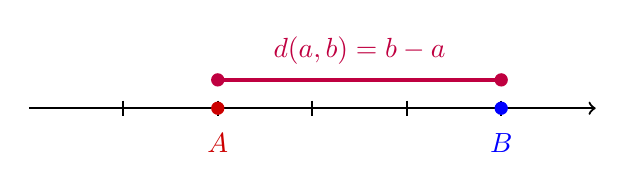
\begin{tikzpicture}[scale=1.2]
			\draw[->, thick] (-1,0) -- (5,0);
			\foreach \x in {0,1,2,3,4} { \draw[thick] (\x,0.08) -- (\x,-0.08); }
			\fill[red!80!black] (1,0) circle (2pt) node[below=2mm] {$A$};
			\fill[blue] (4,0) circle (2pt) node[below=2mm] {$B$};
			\fill[purple] (1,0.3) circle (2pt);
			\fill[purple] (4,0.3) circle (2pt);
			\draw[line width=1.5pt, purple] (1,0.3) -- (4,0.3);
			\node[purple, above=2pt] at (2.5,0.3) {$d(a,b) = \abs{b - a}$};
		\end{tikzpicture}
	\end{center}
\end{df}

\begin{remarque}
	En particulier, pour tout réel $x$, la valeur absolue $\abs{x} = \abs{x - 0} = d(x,0)$ représente la \textbf{distance entre $x$ et l'origine $0$}.
\end{remarque}

\subsection{Équations et inéquations avec valeur absolue}

\begin{prop}[Résolution d'équations $\abs{x - a} = r$]
	Soient $a \in \R$ et $r \geqslant 0$.

	L'équation $\abs{x - a} = r$ signifie que la distance entre $x$ et $a$ est égale à $r$.
	\[
		\abs{x - a} = r \iff \begin{cases}x_1 = a - r \\ x_2 = a + r\end{cases}
	\]
\end{prop}

\begin{ex}
	Résolvons dans $\R$ l'équation $\abs{x - 2} = 3$.

	On cherche les réels $x$ situés à une distance de $3$ du point d'abscisse $2$.

	\begin{center}
		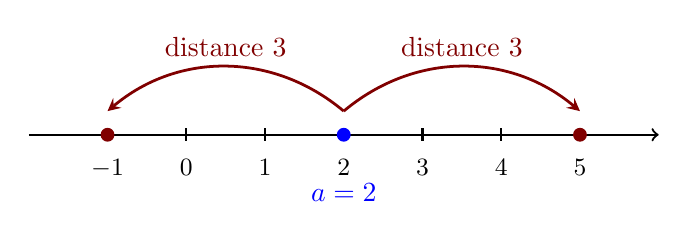
\begin{tikzpicture}[scale=1]
			\draw[->, thick] (-2,0) -- (6,0);
			\foreach \x in {-1,0,1,2,3,4,5} { \draw[thick] (\x,0.08) -- (\x,-0.08) node[below=1mm] {\small $\x$}; }
			\fill[blue] (2,0) circle (2.5pt) node[below=5mm] {$a = 2$};
			\draw[->, >=stealth, line width=1pt, red!50!black] (2,0.3) to[out=140,in=40] node[midway,above] {distance $3$} (-1,0.3);
			\draw[->, >=stealth, line width=1pt, red!50!black] (2,0.3) to[out=40,in=140] node[midway,above] {distance $3$} (5,0.3);
			\fill[red!50!black] (-1,0) circle (2.5pt);
			\fill[red!50!black] (5,0) circle (2.5pt);
		\end{tikzpicture}
	\end{center}

	L'ensemble des solutions est $S = \{-1 \,;\, 5\}$.
\end{ex}

\begin{prop}[Résolution d'inéquations $\abs{x - a} \leqslant r$]
	Soient $a \in \R$ et $r \geqslant 0$.

	L'inéquation $\abs{x - a} \leqslant r$ signifie que la distance entre $x$ et $a$ est inférieure ou égale à $r$.
	\begin{align*}
		\abs{x - a} \leqslant r & \iff x \in \intff{\pa{a - r}}{\pa{a + r}}        \\
		                        & \iff \pa{a - r} \leqslant x \leqslant \pa{a + r}
	\end{align*}
\end{prop}

\begin{ex}
	Résolvons dans $\R$ l'inéquation $\abs{x - 2} \leqslant 3$.

	\textbf{Interprétation :} On cherche les réels $x$ dont la distance à $2$ est inférieure ou égale à $3$.

	\begin{center}
		\begin{tikzpicture}[scale=1]
			% Axe
			\draw[->, thick] (-2.5,0) -- (6.5,0);
			\foreach \x in {-2,-1,0,1,3,4,5,6} { \draw[thick] (\x,0.08) -- (\x,-0.08) node[below=1mm] {\small $\x$}; }

			% Intervalle solution
			\draw[blue, line width=1.5pt, {Bracket[length=4pt, width=13pt]}-{Bracket[length=4pt, width=13pt]}] (-1.03,0) -- (5.03,0);
			\node[blue, above=6pt] at (2,0) {$\intff{-1}{5}$};
			\fill (2,0) circle (2pt) node[below=2mm] {$a = 2$};

			% Flèches de rayon
			\draw[<->, >=stealth, thick, red!50!black] (-1,-1) -- (2,-1) node[midway,below] {$r=3$};
			\draw[<->, >=stealth, thick, red!50!black] (2,-1) -- (5,-1) node[midway,below] {$r=3$};
		\end{tikzpicture}
	\end{center}

	L'ensemble des solutions est l'intervalle $S = \intff{-1}{5}$.
\end{ex}


